% !TEX root = report.tex

\section{Processing Pipeline}
\label{sec:processing_architecture}

In order to provide a complete overview of the approaches that can be followed during this kind of tasks, at a certain point the project will encounter two parallel branches:
\begin{itemize}
	\itemsep0em
	\item one following the more canonical path of classification according to high-level audio features extracted from the clips (used also in speech recognition tasks);
	\item a second one instead moving onto an "unconventional" direction and exploiting Convolutional Neural Networks over the audio spectrograms, that, in recent years have, been found to outperform the canonical way for environmental sounds, even replacing it as the state of the art.
\end{itemize} 
Splitting the analysis into two parts, one is effectively able to compare the two methods in term of speed, stability and accuracy reached, but its implementation requires also the generation of two different new datasets.\\
So, for the first part, a vector of high-level audio features is extracted from the clips, and will represent them during the learning phase for the machine learning models implemented: the main advantage of this method is that each audio file can be simply replaced by a vector with just a few dozen of parameters, resulting in much less memory consumption; so, data are easier to handle and manipulate, at the expenses of some additional preprocessing steps (extraction, dimensionality reduction, regularization). For the second part, instead, the sounds are represented by their power spectrograms, and so the collection of audios leaves space to a set of images, that unfortunately occupy much more memory (obviously depending on their resolution). However this second approach seems to guarantee better performances with very high accuracies, and so it is the preferred one, even if it usually takes much more time to train.\\
Just as a final remark for this part, it can be useful to say that the spectrograms in the second approach can be replaced by their \textit{Melspectrograms}, that basically are the same power spectra, but represented in the Mel scale, which better approximates the human auditory system; however, in the results section it will be shown that both choices lead to similar performances over the dataset studied.\\
The whole procedure is possible thanks to the Python library \textit{Librosa} \cite{mcfee2015librosa}, that provides all the building blocks necessary for music and audio analysis. 


\section{Signals and Features}
\label{sec:model}

As anticipated before, one of the main obstacles in research activities focused on environmental sound classification was the scarcity of large public datasets to analyze and exploit for training models. But it is for this reason that Karol J. Piczak \cite{piczak2015dataset}, realized a collection of sound clips that became one of the two main datasets used to define the state of the art for this research field.\\
The \textbf{ESC-50 dataset} is a labeled collection of 2000 environmental audio recordings suitable for benchmarking methods of environmental sound classification. The dataset consists of 5-second-long recordings \footnote{44.1 kHz, mono, 431 frames, cropped or padded with zeros to reach exactly 5 seconds of duration} organized into 50 semantical classes (with 40 examples per class) loosely arranged into 5 major categories: animals, natural soundscapes and water, human non-speech, interior/domestic sounds and exterior/urban noises. All of these clips have been manually extracted from public field recordings gathered by the \url{Freesound.org} project \footnote{A more thorough description of the dataset is available in the original paper \cite{piczak2015dataset}, while the main folder of the project can be found on github \cite{piczakgithub}.}.\\
As presented in the previous section, one of the peculiarity of this work will be proceeding into two parallel directions, in order to analyze and compare the two main approaches developed and applied so far to solve the problem. For the method exploiting the CNNs, the only preparation required is normalizing the entries of the spectrogram images given in input  \footnote{$(300\times 600)$ .png images} in $[-1,1]$, that is a common step when working with neural networks. For the features' vector approach, instead, the biggest part of the work consist into defining an entire preprocessing procedure aimed to the construction of a reliable high-level representation of the clips. Those steps will be deepened in the following subsections.

\subsection{Features extraction}
\label{sec:features_extraction}
The objective is to define an high-level representation of each sound clip using just a few values, summarizing all the necessary information stored in each audio file. In particular, for this project, the choice fell on the following list of features:
\begin{itemize}
	\itemsep0em
	\item \textbf{spectral centroid}: indicates at which frequency the energy of a spectrum is centered upon or, in other words, where the "center of mass" for a sound is located;
	\item \textbf{spectral roll off}: measure of the signal's shape, represents the frequency at which high frequencies decline to zero;
	\item \textbf{spectral bandwidth}: represents the portion of the spectrum which contains most of the energy of the signal;
	\item \textbf{zero-crossing rate}: rate at which a signal changes from positive to zero to negative or from negative to zero to positive;
	\item \textbf{MFCC}: the Mel-Frequency-Cepstral-Coefficient of a signal are a small set of features (usually about 10/20) which concisely describe the overall shape of a spectral envelope modeling the characteristics of the human voice (according to the Mel scale); only twelve of them are kept (discarding the first one, conventionally) together with their first (\textbf{delta}) and second derivatives (\textbf{delta-delta});
	\item \textbf{chromagram}: typically a 12-element features vector indicating how much energy of each pitch class, \{C, C\#, D, D\#, E, ..., B\}, is present in the signal (usually, it provides a way to describe a similarities between music pieces);
	\item \textbf{energy}: root-mean-square-energy (RMSE) value for each frame, together with the first (\textbf{delta-energy}) and second derivatives (\textbf{delta-delta-energy}) of their logarithms.
\end{itemize}
One could argue that some of them are redundant or even unsuitable for the main objective of the implementation, but later on a Principal Component Analysis will discard all the contribution that effectively are useless, and so computing them at the beginning results in just a negligible increment in the computational time. Moreover, looking at the correlation matrix among those features, and reported in appendix \ref{app:correlation_matrix}, one can find additional justifications for this choice.\\
Notice that the list above is constituted by \textit{frame features}, in the sense that each quantity will contribute with one (or more) values for every frame in the clip (431), and so in the end one will have to deal with entire distributions, rather than single vectors. The first and also the most immediate solution, that one can think about, is representing each feature with its mean across all the frames, leading to vectors of overall size 55. But this will be shown to be a suboptimal attempt because there are many audio files whose features distributions are not very regular neither symmetric, like shown in figure \ref{fig:ex_distrib}, and so the mean alone is no more representing a good estimator for them: to take into account the dispersion of the data, one should rely also on other statistical estimators like the standard deviation.
\begin{figure}[!h]
	\centering
	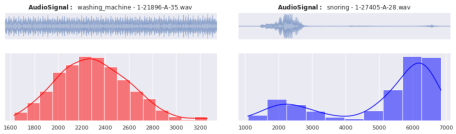
\includegraphics[width=0.47\textwidth]{pictures/ex_distrib.pdf}
	\caption{Spectral centroid distributions for two different sound clips.}
	\label{fig:ex_distrib}
\end{figure}
So the final choice fell on constructing, for each clip, a vector containing the mean and the standard deviation across the frames, for all the features listed above, for a total of 110 elements.

\subsection{Silent Elimination}
\label{sec:windowing}
A further preprocessing step that can be implemented is the detection of silent windows in the clips.
\begin{figure}[!h] 
	\centering
	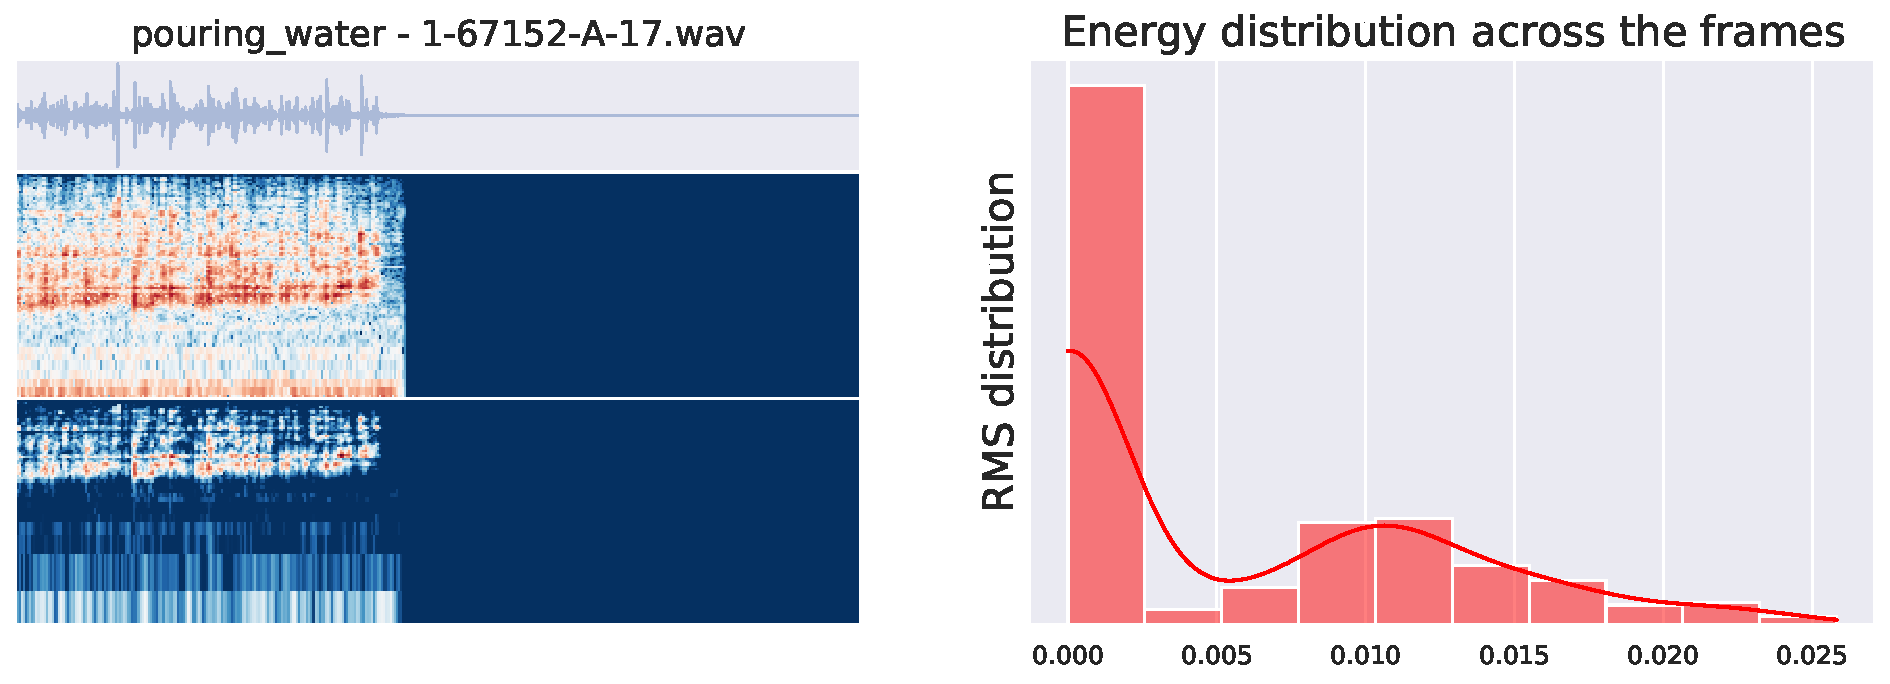
\includegraphics[width=0.47\textwidth]{pictures/silent_ex.pdf}
	\caption{Example of a clip with a large fraction of silence.}
	\label{fig:silent_ex}
\end{figure}
As can be noticed in picture \ref{fig:silent_ex}, there are some sounds which have been padded with zeros to reach the five second length, or maybe they just alternate parts of noises and parts of silence. This can be a problem in the final classification, because the features distributions, represented just by their mean and standard deviation, will result strongly shifted towards the zeros measured during those periods of silence, losing, then, much of their regularity. One possibility to deal with this problem could be "forgetting" about zeros when computing the statistical variables of the features: in this way the mean would result just re-scaled, while the standard deviation would be affected much more. Hence the final accuracy is effectively increased, but the problem is that we are improving the capability of the model when distinguishing among short sounds, but at the same time we are losing information about repetitive sounds, like some animal noises. A possible trade-off between the two situations has been found defining a further step, not on the clips, but directly on the features, according to which if the program is able to identify fix-sized windows of silence, using the energy of the spectrum as a discriminator, those (non-overlapping) windows can be "forgotten" during the calculation. After several tests, it turned out that the optimal windows' size was 0.5 seconds.

\subsection{Audio Augmentation}
\label{sec:audio_augmentation}
The dataset used in this analysis is composed just by 2000 clips for 50 different classes: not enough to train a good classifier nor to construct a reliable statistics of the results.
One possible solution to this is data augmentation, i.e. increasing the amount of clips available, adding slightly modified copies of already existing data or newly created ones. In this way, at least theoretically, the possibility of overfitting will be reduced, making the models able to generalize better. Starting from the original audio files, four new folders, each containing 2000 clips, have been generated, applying one of the available augmentation techniques (inspired by the ones suggested by Salomon and Bello \cite{salamon_bello}, and by the work of Nanni, Maguolo and Paci \cite{animal_augmentation}):
\begin{itemize}
	\itemsep0em
	\item \textit{Background Noise}: mix the audio sample with some gaussian noise multiplied by a regularization factor, that is calibrated to avoid such noise to overcome too much the original sound.
	\item \textit{Time Shifting}: sounds should be invariant under time shifting, and so new clips are generated in this way, padding with zeros the part that has been moved.
	\item \textit{Pitch Shifting}: sound recording technique in which the original pitch of a sound is raised or lowered and, according to Salomon and Bello \cite{salamon_bello}, is particularly beneficial for the augmentation and should deserve a separate analysis.
	\item \textit{Time Stretching}: just slowing down or speeding up the audio samples.
\end{itemize}

However, even if the data augmentation step has been reported and implemented, its efficiency will be seriously questioned in the results section, since it will be shown that traditional audio augmentation techniques are not compatible with the approaches followed for environmental sound classification.


\section{Learning Framework}
\label{sec:learning_framework}

Again, this section is divided into two parts, following the two different approaches implemented: the first one exploiting several machine learning classifiers trained with the vectors constructed in section \ref{sec:features_extraction}, and the second one utilizing CNNs to classify spectrograms. 

\subsection{Features Classification}
\label{sec:features_classification}
There is a "problem" with the ESC-50 dataset: it composed by just 2000 clips, which is never enough to train properly a 50-classes classifier! Also splitting the clips in a train-validation-test sets is not so recommended, because there isn't enough data to construct a significative statistics. A possible solution to all these problems have been found in a technique (suggested also inside the library \textit{sklearn}) called \textbf{nested cross-validation}, presented in appendix \ref{app:nested_CV}.\\
Then, it's all about figuring out which kind of machine learning models can effectively be trained with success over the clips collected in ESC-50 (or, better, on the features vectors extracted from them). This project started studying the application of four different "canonical" classifiers (provided by \textit{sklearn}) for some reasonable combinations of hyperparameters:
\begin{itemize}
	\itemsep0em
	\item a \textbf{Random Forest};
	\item a \textbf{Multi-Layer Perceptron};
	\item a \textbf{K-Neighbors Classifier};
	\item a \textbf{Support Vector Machine}.
\end{itemize}

Moreover, before feeding them with the (nested) folds created splitting the dataset, the vectors needed a final preprocessing step, made possible via a data-\textit{pipeline} implementing the following three operations:
\begin{enumerate}
	\item standardization of the features (via a \textit{StandardScaler});
	\item Principal Component Analysis (whose effects will be studied in appendix \ref{app:dim_reduction});
	\item label encoding (numerical or one-hot depending on the model).
\end{enumerate}

In addition to the four models listed above, also a feed-forward neural network has been built, with the purpose of having a more customizable architecture and the possibility of monitoring the behavior of the loss across the epochs. Such network is structured in the following way:
\begin{itemize}
	\itemsep0em
	\item 3 layers with $1024 \to 512 \to 50$ nodes;
	\item \textit{PreLU} as activation function;
	\item Dropouts and BatchNormalizations;
	\item \textit{Categorical Cross-Entropy} as loss function.
\end{itemize}

And now it's just about running the training procedure for several parameters/methods/models and complete all the studies necessary to find the combination that will guarantee the higher accuracy and stability.


\subsection{Spectrograms Classification}
\label{sec:spectrograms_classification}
One of the main differences between the previous methods and the spectrograms classification is the memory required: in the latter case, in fact, we need to store one image per clip, and an image is much bigger than a vector with just one hundred of samples. We will, usually have to deal with datasets larger than 1 Gb, with the consequent difficulties in loading and manipulating them. For this reason, using a binary file format for data storage can bring to a significant improvement in term of performances, and consequently also on the model's training time. Binary data, in fact, takes up less space on disk, especially when compressed, and can be read in a much more efficient way. \textit{Tensorflow} has developed its own binary storage format, that is the \textit{TFRecord} \footnote{\href{https://medium.com/mostly-ai/tensorflow-records-what-they-are-and-how-to-use-them-c46bc4bbb564}{Tensorflow Records? What they are and how to use them}} format, gifted of a lot of preprocessing functionalities and the possibility of loading from the disk and processing, only the data required at that particular time, allowing for an efficient way to deal with large datasets. Unfortunately, this way of proceeding forbid the usage of cross validation, but at the expenses of a small further preparation step (simply generating $k$ tfrecord files splitting the clips by label before loading them) one can still exploit the method to compensate the scarcity of data. After having determined how to handle such large quantity of images, is time to select the machine learning classifier, and the choice fell on Convolutional Neural Networks, whose high performances has already been proved by several other studies. Apparently, in fact, the possibility of learning local structures from a bidimensional input outperforms the previous approaches, mainly based on the extraction of vectors of features, directly from the raw audio files.\\
Then it's all about selecting a proper architecture to fit the spectrograms of the clips. The following choices have been dictated by a long research phase to achieve the best performances in term of accuracy and stability:
\begin{itemize}
	\itemsep0em
	\item labels are one-hot encoded;
	\item the loss function is the \textit{Categorical Crossentropy} while the first metric is the \textit{Categorical Accuracy};
	\item the optimizer is \textit{Adamax}, that apparently works better than \textit{Adam} for almost any architecture studied;
	\item the learning rate is quite small, $lr = 0.00005$, that turned out to represent a good tradeoff between training speed, stability and accuracy; an adaptive learning rate is possible, but apparently does not affect very well the stability of the convergence.
\end{itemize}
The architecture used is represented in figure \ref{fig:cnn_architecture}, in which we can distinguish 3 convolutional blocks, characterized by an increasing number of filters and a progressive reduction of the kernel size, in order to simplify the learning of features that will be smaller and smaller as they pass through the network. In fact, at the end of each block there is a \textit{MaxPooling} layer with the purpose of reducing the size of the input images: particularly relevant is the first pooling layer, which strides are set to $(2,4)$, in such a way that images can be reshaped from a rectangular to a square form. Then, there is a fourth fully-connected block that ends with a layer composed by exactly 50 neurons, corresponding to the 50 possible classes of the images. As activation function the \textit{PReLU} has been selected for all the layers, since it helps the network to prevent vanishing gradients and does not increase too much the time necessary to process the epochs. This architecture has been inspired by several Convolutional models and canonical structures that have been used for this kind of problems, and in particular to AlexNet \cite{alexnet} and VGG16 \cite{vgg16}, even if those ones were mainly designed for the dataset ImageNet \cite{imagenet}.
\begin{figure}[!h]
	\centering
	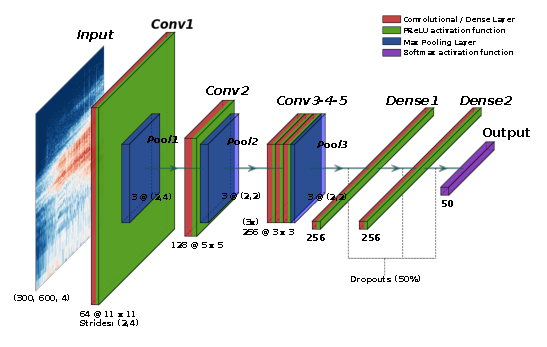
\includegraphics[width=0.45\textwidth]{pictures/cnn_architecture.pdf}
	\caption{Architecture of the Convolutional Neural Network.}
	\label{fig:cnn_architecture}
\end{figure}

As last trial to reach a decent accuracy, a more complex architecture has been built merging a feedforward network and the convolutional described above. Its schematic representation is left at figure \ref{fig:finalnet_architecture}: the idea is using for each clip a double input, made by the features vector and the spectrogram, that will proceed independently one of the other, trough the branches of the network, and the end a unique layer of 50 nodes will predict the class biased by both branches.

\begin{figure}[!h]
	\centering
	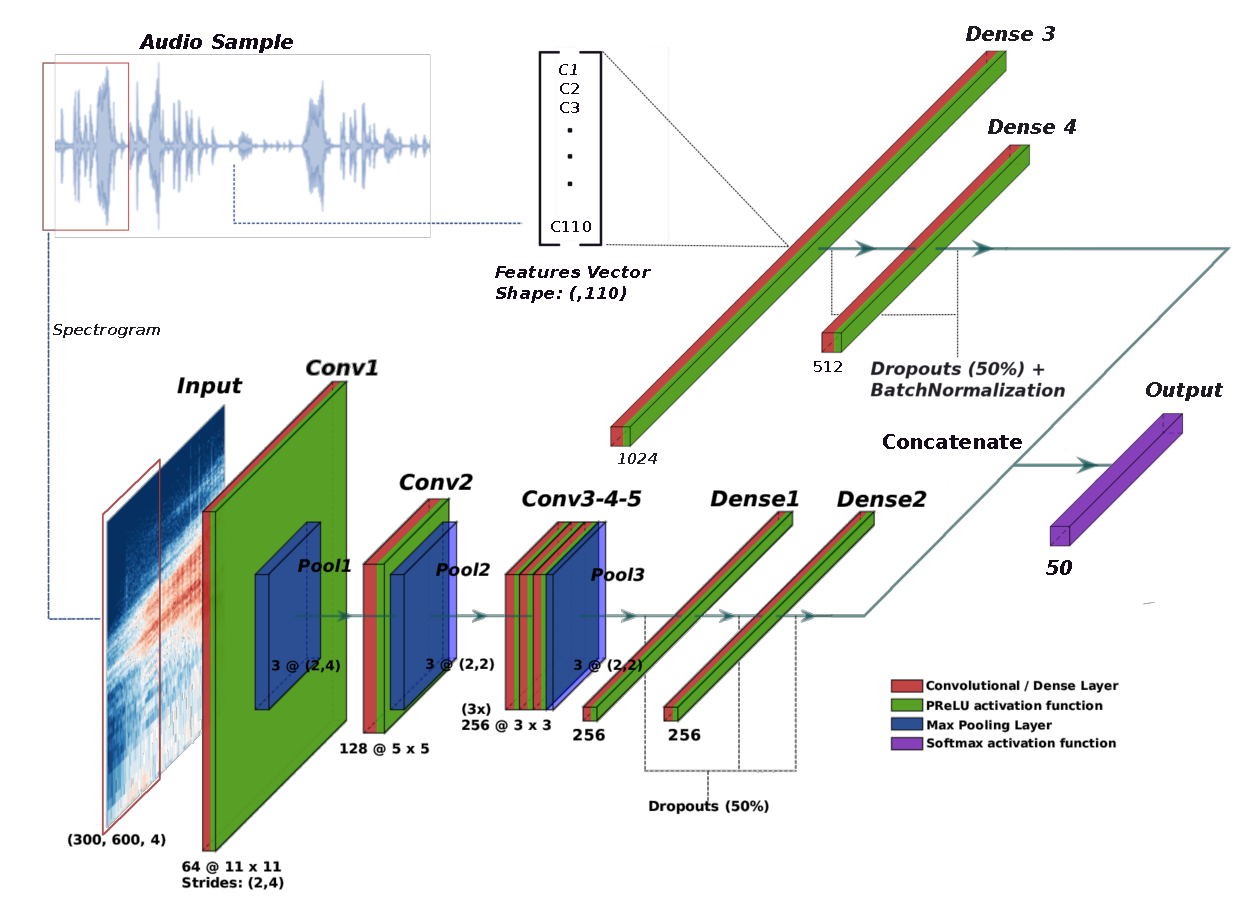
\includegraphics[width=0.45\textwidth]{pictures/finalnet_architecture.pdf}
	\caption{Architecture of the composite Neural Network (FFN + CNN).}
	\label{fig:finalnet_architecture}
\end{figure}



